\documentclass[11pt,letterpaper]{article}
\usepackage[utf8]{inputenc}
\usepackage[T1]{fontenc}
\usepackage{lmodern}
\usepackage[margin=1in]{geometry}
\usepackage{amsmath,amssymb,amsfonts,amsthm}
\usepackage{booktabs}
\usepackage{microtype}
\usepackage{enumitem}
\usepackage{fancyhdr}
\usepackage{titlesec}
\usepackage{xcolor}
\usepackage{tikz}
\usepackage{pgfplots}
\usepackage{mdframed}
\usepackage[hidelinks,colorlinks=true,linkcolor=SlateBlue,citecolor=SlateBlue,urlcolor=Terracotta]{hyperref}

\pgfplotsset{compat=1.18}
\usetikzlibrary{arrows.meta,positioning,calc,patterns,decorations.pathreplacing}

\definecolor{SlateBlue}{HTML}{1E293B}
\definecolor{Terracotta}{HTML}{C2410C}
\definecolor{ForestGreen}{HTML}{15803D}
\definecolor{LightSlate}{HTML}{F8FAFC}
\definecolor{BorderGray}{HTML}{CBD5E1}
\definecolor{LightTerracotta}{HTML}{FFF7ED}
\definecolor{CourseBlue}{HTML}{0072B2}
\definecolor{CourseOrange}{HTML}{D55E00}
\definecolor{CourseTeal}{HTML}{009E73}
\definecolor{CoursePurple}{HTML}{CC79A7}
\definecolor{CourseAmber}{HTML}{E69F00}

\titleformat{\section}{\normalfont\Large\bfseries\color{SlateBlue}}{\thesection}{1em}{}[\titlerule]
\titleformat{\subsection}{\normalfont\large\bfseries\color{SlateBlue}}{\thesubsection}{1em}{}
\titleformat{\subsubsection}{\normalfont\normalsize\bfseries\color{Terracotta}}{\thesubsubsection}{1em}{}

\pagestyle{fancy}
\fancyhf{}
\renewcommand{\headrulewidth}{0.4pt}
\renewcommand{\footrulewidth}{0.4pt}
\fancyhead[L]{\small\scshape\color{SlateBlue}\leftmark}
\fancyhead[R]{\small\color{SlateBlue}Principles of Economics}
\fancyfoot[C]{\thepage}

\newmdenv[
  linecolor=Terracotta,
  linewidth=1.5pt,
  backgroundcolor=LightTerracotta,
  innertopmargin=10pt,
  innerbottommargin=10pt,
  innerrightmargin=12pt,
  innerleftmargin=12pt,
  roundcorner=4pt,
  skipabove=12pt,
  skipbelow=12pt
]{coreprinciple}

\newmdenv[
  linecolor=SlateBlue,
  linewidth=1.5pt,
  backgroundcolor=LightSlate,
  innertopmargin=10pt,
  innerbottommargin=10pt,
  innerrightmargin=12pt,
  innerleftmargin=12pt,
  roundcorner=4pt,
  skipabove=12pt,
  skipbelow=12pt
]{casestudy}

\newenvironment{examplecase}[1]{%
  \begin{casestudy}
  \boxheader{SlateBlue}{#1}
  \vspace{0.4em}
}{%
  \end{casestudy}
}

\newmdenv[
  linecolor=BorderGray,
  linewidth=1pt,
  backgroundcolor=white,
  innertopmargin=10pt,
  innerbottommargin=10pt,
  innerrightmargin=12pt,
  innerleftmargin=12pt,
  roundcorner=4pt,
  skipabove=12pt,
  skipbelow=12pt
]{takeaways}

\newcommand{\boxheader}[2]{{\noindent\bfseries\color{#1}\Large #2}\vspace{0.4em}\par}

% ==============================================================================
% TikZ & PGFPlots Global Configuration and Economics Styling
% ==============================================================================

\usepackage{tikz}
\usepackage{pgfplots}
\pgfplotsset{compat=1.18}

% TikZ Libraries
\usetikzlibrary{
    arrows.meta,
    positioning,
    calc,
    shapes.geometric,
    patterns,
    decorations.pathreplacing,
    intersections
}

% Common Economics TikZ Styles
\tikzset{
    % Axes and Structural Lines
    econ axis/.style={->, >=Stealth, thick, color=SlateBlue!90!black},
    econ grid/.style={thin, dashed, color=gray!30},
    econ guide/.style={dashed, color=gray!60, thin},
    % Curves and Functions
    demand curve/.style={very thick, color=SlateBlue},
    supply curve/.style={very thick, color=Terracotta},
    mb curve/.style={very thick, color=SlateBlue},
    mc curve/.style={very thick, color=Terracotta},
    % Points and Highlights
    econ point/.style={circle, fill=SlateBlue!90!black, inner sep=1.8pt},
    econ highlight/.style={fill=Terracotta!20, opacity=0.5},
    % Annotations
    econ label/.style={font=\small\sffamily, align=center},
    econ annotation/.style={font=\footnotesize\itshape, color=SlateBlue!80!black}
}

% PGFPlots Standard Economics Style
\pgfplotsset{
    econ diagram/.style={
        axis lines=left,
        xlabel style={at={(ticklabel* cs:1)}, anchor=north west, font=\small\bfseries},
        ylabel style={at={(ticklabel* cs:1)}, anchor=south east, font=\small\bfseries},
        label style={font=\small},
        tick label style={font=\small},
        grid=none,
        enlargelimits=false,
        axis line style={->, >=Stealth, thick, color=SlateBlue!90!black}
    }
}

\usepackage{tcolorbox}

\begin{document}

\title{\Huge\bfseries\color{SlateBlue} Chapter 9: Fiscal Policy, Automatic Stabilizers, and Sovereign Debt}
\author{\large Principles of Macroeconomics Curriculum}
\date{2026}
\maketitle

\thispagestyle{plain}

\begin{abstract}
This chapter provides a rigorous, pedagogical treatment of Chapter 9: Fiscal Policy, Automatic Stabilizers, and Sovereign Debt, benchmarked to standard principles curriculum.
\end{abstract}

\tableofcontents
\vspace{1.5em}
\hrule
\vspace{1.5em}

% -----------------------------------------------------------------------------
% Section 9.1: Discretionary Fiscal Policy and Multipliers in AD-AS
% -----------------------------------------------------------------------------
\section{Discretionary Fiscal Policy and Multipliers in AD-AS}

\subsection*{1. Conceptual Introduction}
\textbf{Fiscal policy} refers to government decisions regarding the level of government purchases ($G$) and net taxes ($T$), enacted deliberately by Congress and the President to influence macroeconomic activity. When the economy suffers from a severe recessionary gap, **expansionary fiscal policy**—increasing government purchases or cutting taxes—shifts aggregate demand rightward to close the output gap. Conversely, during an overheating inflationary boom, **contractionary fiscal policy**—cutting government spending or raising taxes—shifts aggregate demand leftward.

Evaluating fiscal policy requires accounting for the **spending multiplier** (analyzed in Chapter 7) and the **price-level response** in AD-AS. In the Keynesian cross model with fixed prices, a $\$100\text{ billion}$ increase in government purchases expands output by $\$100\text{B} \times k_G$. In the AD-AS model, because the aggregate supply curve slopes upward, part of the expansionary boost spills over into a higher price level rather than pure real output growth—making the effective short-run fiscal multiplier smaller than the fixed-price multiplier.

\subsection*{2. Visual Representation}
Figure~\ref{fig:fiscal_policy_adas} illustrates expansionary fiscal policy shifting aggregate demand rightward from $AD_1$ to $AD_2$, closing a recessionary gap and moving the economy from $E_1$ to $E_2$.

\begin{tcolorbox}[colback=yellow!10!white,colframe=orange!80!black,title=\textbf{Clear It Up: The Lags of Fiscal Policy}]
Fiscal policy is subject to three major administrative time lags that can impair its timing: (1) the **recognition lag** (identifying that a recession has begun), (2) the **legislative lag** (debating and passing tax or spending bills in Congress), and (3) the **implementation lag** (delivering funds and starting infrastructure projects). A well-intended fiscal stimulus package can sometimes arrive just as the economy is already recovering naturally.
\end{tcolorbox}

\begin{figure}[htbp]
\centering
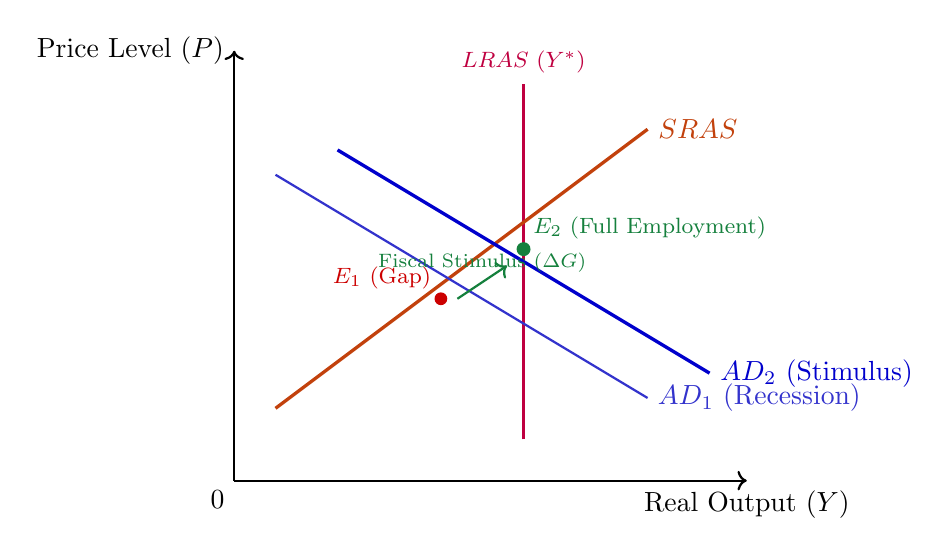
\begin{tikzpicture}[scale=1.05]
    % Axes
    \draw[->, thick] (0,0) -- (6.2,0) node[below] {Real Output ($Y$)};
    \draw[->, thick] (0,0) -- (0,5.2) node[left] {Price Level ($P$)};
    \node[below left] at (0,0) {$0$};

    % LRAS at Y* (x = 3.5)
    \draw[very thick, color=purple] (3.5,0.5) -- (3.5,4.8) node[above, font=\footnotesize] {$LRAS$ ($Y^*$)};

    % SRAS: P = 0.5 + 0.75Q -> (0.5,0.875) to (5.0,4.25)
    \draw[very thick, color=Terracotta] (0.5,0.875) -- (5.0,4.25) node[right] {$SRAS$};

    % AD1 (Recessionary intersection at Y1=2.5): P = 4.0 - 0.6Q
    \draw[thick, color=blue!60!gray] (0.5,3.7) -- (5.0,1.0) node[right] {$AD_1$ (Recession)};
    % AD2 (Stimulus intersection at Y*=3.5): P = 4.75 - 0.6Q
    \draw[very thick, color=blue!80!black] (1.25,4.0) -- (5.75,1.3) node[right] {$AD_2$ (Stimulus)};

    % E1(2.5, 2.2)
    \filldraw[red!80!black] (2.5,2.2) circle (2pt) node[above left, font=\footnotesize] {$E_1$ (Gap)};
    % E2(3.5, 2.8)
    \filldraw[ForestGreen] (3.5,2.8) circle (2.2pt) node[above right, font=\footnotesize] {$E_2$ (Full Employment)};

    \draw[->, thick, color=ForestGreen] (2.7,2.2) -- node[above, font=\scriptsize] {Fiscal Stimulus ($\Delta G$)} (3.3,2.6);
\end{tikzpicture}
\caption{Expansionary Fiscal Policy in AD-AS. Increasing government purchases shifts $AD_1 \to AD_2$, moving output from recessionary $E_1$ to full-employment potential output $E_2$.}
\label{fig:fiscal_policy_adas}
\end{figure}

\subsection*{3. Real-World Application: The American Recovery and Reinvestment Act (ARRA)}
In response to the 2008 financial crisis, the federal government enacted the $\$831\text{ billion}$ ARRA stimulus package, combining infrastructure grants, state fiscal relief, and temporary tax cuts. Economists debated the exact size of the empirical multiplier, highlighting how open-economy leakages and debt-induced interest rate reactions dampen fiscal stimulus.

## 4. Mathematical Foundation (Algebra Level)
The government purchases multiplier in a closed model with income taxes $t$ is:
\begin{equation}
k_G = \frac{1}{1 - c(1 - t)}
\end{equation}

\noindent\textbf{Worked Problem:}
An economy is stuck in a recessionary gap with actual output $Y = \$20.0\text{ trillion}$ and Potential GDP $Y^* = \$22.0\text{ trillion}$ (a $\$2.0\text{ trillion}$ output gap). The marginal propensity to consume is $c = 0.8$ and the income tax rate is $t = 0.25$ (so the effective spending multiplier is $k_G = \frac{1}{1 - 0.8(0.75)} = \frac{1}{0.4} = 2.5$).
\begin{enumerate}
    \item Calculate the exact increase in government purchases ($\Delta G$) required to close the $\$2.0\text{ trillion}$ output gap.
    \item Alternatively, calculate the required tax cut ($\Delta T$) needed to close the gap, using the tax multiplier $k_T = \frac{-c(1-t)}{1 - c(1-t)} = \frac{-0.6}{0.4} = -1.5$.
\end{enumerate}

\noindent\textbf{Step-by-Step Breakdown:}
\begin{enumerate}
    \item \textbf{Compute Required Government Purchases Increase ($\Delta G$):}
    \[
    \Delta Y^* = k_G \cdot \Delta G \implies \$2.0\text{T} = 2.5 \cdot \Delta G \implies \Delta G = \frac{\$2.0\text{T}}{2.5} = \mathbf{\$0.8\text{ trillion}\ (\$800\text{B})}
    \]

    \item \textbf{Compute Required Tax Cut ($\Delta T$):}
    \[
    \Delta Y^* = k_T \cdot \Delta T \implies \$2.0\text{T} = -1.5 \cdot \Delta T \implies \Delta T = \frac{\$2.0\text{T}}{-1.5} \approx \mathbf{-\$1.33\text{ trillion}}
    \]
\end{enumerate}
\textbf{Conclusion:} Closing the gap requires either $\$800\text{ billion}$ in new government spending or a $\$1.33\text{ trillion}$ tax cut (since households save part of any tax cut rather than spending it all).

% -----------------------------------------------------------------------------
% Section 9.2: Automatic Stabilizers and Budget Deficits vs. Debt
% -----------------------------------------------------------------------------
\section{Automatic Stabilizers and Budget Deficits vs. Debt}

\subsection*{1. Conceptual Introduction}
Not all fiscal stabilization requires new congressional legislation. Modern economies feature built-in \textbf{automatic stabilizers}—fiscal rules and tax structures that automatically expand government borrowing during recessions and contract borrowing during booms without requiring a vote:
\begin{itemize}
    \item \textbf{Progressive Income Taxes:} As household incomes and corporate profits fall during a recession, tax collections drop automatically, cushioning disposable income.
    \item \textbf{Unemployment Insurance and Welfare Transfers:} When workers lose jobs during a downturn, unemployment insurance payouts rise automatically, supporting consumer spending.
\end{itemize}

It is also essential to keep fiscal flows and stocks distinct:
\begin{itemize}
    \item \textbf{Budget Deficit (Flow):} The excess of government outlays over tax revenues during a single fiscal year.
    \item \textbf{National Debt (Stock):} The accumulated total of all past annual budget deficits minus surpluses, representing total outstanding government liabilities.
\end{itemize}

## 2. Visual Representation
Figure~\ref{fig:automatic_stabilizers} illustrates how progressive tax brackets and unemployment benefits create a countercyclical budget balance—generating automatic deficits during recessions and surpluses during expansions.

\begin{figure}[htbp]
\centering
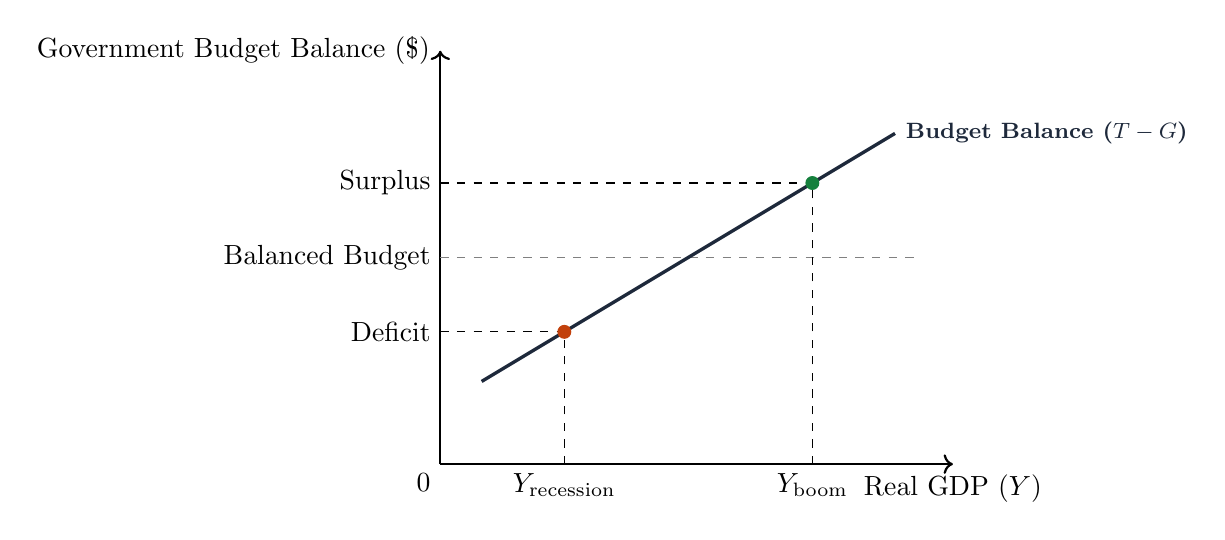
\begin{tikzpicture}[scale=1.05]
    % Axes
    \draw[->, thick] (0,0) -- (6.2,0) node[below] {Real GDP ($Y$)};
    \draw[->, thick] (0,0) -- (0,5.0) node[left] {Government Budget Balance (\$)};
    \node[below left] at (0,0) {$0$};

    % Zero balance line
    \draw[dashed, gray] (0,2.5) node[left, black] {Balanced Budget} -- (5.8,2.5);

    % Budget balance line sloping upward with income Y: Surplus at high Y, Deficit at low Y
    \draw[very thick, color=SlateBlue] (0.5,1.0) -- (5.5,4.0) node[right, font=\footnotesize\bfseries] {Budget Balance ($T - G$)};

    % Recession point R at low Y
    \draw[dashed] (1.5,0) node[below] {$Y_{\text{recession}}$} -- (1.5,1.6);
    \draw[dashed] (0,1.6) node[left] {Deficit} -- (1.5,1.6);
    \filldraw[Terracotta] (1.5,1.6) circle (2.2pt);

    % Boom point B at high Y
    \draw[dashed] (4.5,0) node[below] {$Y_{\text{boom}}$} -- (4.5,3.4);
    \draw[dashed] (0,3.4) node[left] {Surplus} -- (4.5,3.4);
    \filldraw[ForestGreen] (4.5,3.4) circle (2.2pt);
\end{tikzpicture}
\caption{Automatic Stabilizers and the Government Budget Balance. Progressive taxes and transfer programs cause the government budget balance to move countercyclically—running automatic deficits during recessions and automatic surpluses during economic booms.}
\label{fig:automatic_stabilizers}
\end{figure}

\subsection*{3. Real-World Application: St. Louis Fed FRED Series `FYFSD`}
St. Louis Fed FRED series `FYFSD` (Federal Surplus or Deficit[-] as a Percentage of GDP, annual) tracks U.S. federal budget outcomes across decades. Reviewing `FYFSD` reveals deep automatic deficits during the 2008 financial crisis and the 2020 pandemic as tax receipts fell and unemployment insurance transfers surged.

## 4. Mathematical Foundation (Algebra Level)
The government budget balance ($BB$) as a function of national income $Y$ is:
\begin{equation}
BB(Y) = T(Y) - G = (T_0 + tY) - G
\end{equation}

\noindent\textbf{Worked Problem:}
Suppose a government's fixed spending is $G = \$600\text{ billion}$, autonomous taxes are $T_0 = \$100\text{ billion}$, and the marginal income tax rate is $t = 0.20$.
\begin{enumerate}
    \item Write the budget balance function $BB(Y)$.
    \item Compute the budget balance if national income is at recessionary level $Y_1 = \$2{,}000\text{ billion}$ versus full-employment level $Y_2 = \$3{,}000\text{ billion}$.
\end{enumerate}

\noindent\textbf{Step-by-Step Breakdown:}
\begin{enumerate}
    \item \textbf{Write the Budget Balance Equation:}
    \[
    BB(Y) = (100 + 0.20Y) - 600 = \mathbf{-500 + 0.20Y}
    \]

    \item \textbf{Compute Budget Balance at $Y_1 = \$2{,}000\text{B}$ and $Y_2 = \$3{,}000\text{B}$:}
    \[
    BB(\$2{,}000) = -500 + 0.20(2{,}000) = -500 + 400 = \mathbf{-\$100\text{ billion}\ (\text{Deficit})}
    \]
    \[
    BB(\$3{,}000) = -500 + 0.20(3{,}000) = -500 + 600 = \mathbf{+\$100\text{ billion}\ (\text{Surplus})}
    \]
\end{enumerate}
\textbf{Conclusion:} Automatic stabilizers generate a $\$100\text{ billion}$ deficit during a downturn and a $\$100\text{ billion}$ surplus during a boom.

\begin{tcolorbox}[colback=blue!5!white,colframe=blue!75!black,title=\textbf{Optional Advanced Section: Debt-to-GDP Dynamics Equation}]
\small
\emph{Note for Economics Majors and Quantitative Students:}
Let $D_t$ be the debt-to-GDP ratio, $d_t$ be the primary deficit-to-GDP ratio, $r$ be the real interest rate, and $g$ be the real GDP growth rate. The law of motion for the debt-to-GDP ratio is:
\[
D_t - D_{t-1} \approx d_t + \left( \frac{r - g}{1 + g} \right) D_{t-1}
\]
If economic growth $g$ exceeds the real interest rate $r$, the debt-to-GDP ratio shrinks over time even when running a small primary budget deficit ($d_t > 0$).
\end{tcolorbox}

\end{document}